%======================================================================
\chapter{A pseudo-arc in the plane}\label{ch:plane}
%======================================================================

By Theorem~\ref{thm:desc-pseudoarc}, to find a pseudo-arc in $\R^2$ it suffices to construct a
description in $\R^2$, from a point $P$ to a point $Q\neq P$, all of whose links lie in a compact
set. This chapter does so with explicit formulas. The construction is iterative: each level is
the image of the standard chain under a homeomorphism of the plane, and the next level is
obtained by composing with one more explicit homeomorphism, which ``folds'' a long, thin copy
of the standard chain inside the current one according to the stuttered Bing pattern.

Recall that $\R^2$ carries the maximum metric, so that $\diam\big([a,a']\times[b,b']\big)=
\max(a'-a,b'-b)$, and that $[n]=\set{0,\dots,n-1}$.

\section{Standard chains, zones and boxes}\label{sec:std}

\begin{definition}\label{def:std-sets}
For $j\in\N$ and $m\ge1$ define the following subsets of $\R^2$:
\begin{align*}
S_j&=(2j,\,2j+3)\times(0,1) &&\text{(standard link)},\\
Z_j&=[2j+\tfrac85,\,2j+\tfrac{17}5]\times[0,1] &&\text{(zone)},\\
A&=[\tfrac98,\,\tfrac{15}8]\times[\tfrac14,\tfrac34] &&\text{(first box)},\\
B_m&=[2m-\tfrac78,\,2m-\tfrac18]\times[\tfrac14,\tfrac34] &&\text{(last box)},\\
R_m&=[0,\,2m+1]\times[0,1] &&\text{(region)}.
\end{align*}
\end{definition}

\formal{\lean{HPC.Plane.stdRect}, \lean{HPC.Plane.zone}, \lean{HPC.Plane.boxA},
\lean{HPC.Plane.boxB}, \lean{HPC.Plane.region} (\lean{HPC/Plane/StdChain.lean}).}

\begin{figure}[ht]
\centering
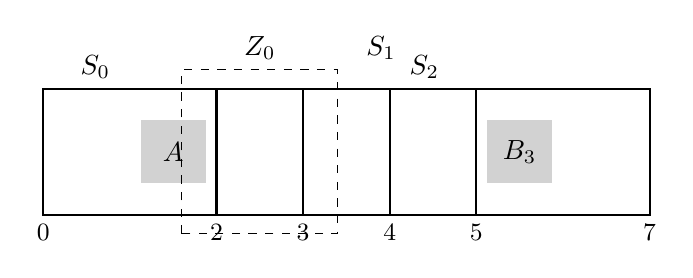
\begin{tikzpicture}[x=1.1cm,y=1.6cm]
  \draw[thick] (0,0) rectangle (3,1);
  \draw[thick] (2,0) rectangle (5,1);
  \draw[thick] (4,0) rectangle (7,1);
  \fill[gray!35] (1.125,0.25) rectangle (1.875,0.75);
  \fill[gray!35] (5.125,0.25) rectangle (5.875,0.75);
  \draw[dashed] (1.6,-0.15) rectangle (3.4,1.15);
  \node at (1.5,0.5) {$A$};
  \node at (5.5,0.5) {$B_3$};
  \node[below] at (0,0) {\small $0$};
  \node[below] at (2,0) {\small $2$};
  \node[below] at (3,0) {\small $3$};
  \node[below] at (4,0) {\small $4$};
  \node[below] at (5,0) {\small $5$};
  \node[below] at (7,0) {\small $7$};
  \node[above] at (0.6,1) {$S_0$};
  \node[above] at (4.4,1) {$S_2$};
  \node[above] at (3.9,1.15) {$S_1$};
  \node[above] at (2.5,1.15) {$Z_0$};
\end{tikzpicture}
\caption{The standard chain $S_0,S_1,S_2$ (open rectangles of height $1$), the zone $Z_0$
(dashed; it has height $1$ and is drawn slightly enlarged), and the boxes $A$ and $B_3$ (shaded).}
\label{fig:std}
\end{figure}

\begin{lemma}\label{lem:std-facts}
Let $m\ge1$.
\begin{enumerate}[label=(\alph*)]
\item\label{sf:chain} $(S_0,\dots,S_{m-1})$ is a chain (Example~\ref{ex:std-chain}); $\cl{S_j}=
[2j,2j+3]\times[0,1]$ and $\diam S_j=3$.
\item\label{sf:zone} $\diam Z_j=\frac95\le2$, and $Z_j\supseteq\cl{S_j\cap S_{j+1}}=[2j+2,2j+3]\times
[0,1]$.
\item\label{sf:A} $A\subseteq S_0$ and $A\cap S_j=\emptyset$ for $j\ge1$.
\item\label{sf:B} $B_m\subseteq S_{m-1}$ and $B_m\cap S_j=\emptyset$ for $j\le m-2$.
\item\label{sf:R} $\cl{S_j}\subseteq R_m$ for $j<m$; $R_m$, $A$, $B_m$ and $Z_j$ are compact.
\end{enumerate}
\end{lemma}

\begin{proof}
All are immediate from the coordinates. For~\ref{sf:A}: $1<\frac98$ and $\frac{15}8<2$, so
$A\subseteq(0,3)\times(0,1)$, while points of $S_j$ ($j\ge1$) have first coordinate $>2j\ge2$.
For~\ref{sf:B}: $2m-2<2m-\frac78$ and $2m-\frac18<2m+1$; and points of $S_j$ with $j\le m-2$ have
first coordinate $<2j+3\le2m-1<2m-\frac78$.
\end{proof}

\begin{definition}[Tame chains]\label{def:tame}
For a homeomorphism $\Phi\colon\R^2\to\R^2$ and $m\ge1$, the \emph{tame chain} $T(\Phi,m)$ is
$(\Phi(S_0),\dots,\Phi(S_{m-1}))$.
\end{definition}

Since $\Phi$ maps open sets to open sets and $\Phi(S_i)\cap\Phi(S_j)\neq\emptyset$ if and only if
$S_i\cap S_j\neq\emptyset$, a tame chain is a chain. Its links are bounded:
$\Phi(S_j)\subseteq\Phi(\cl{S_j})$, which is compact. And $\cl{\Phi(S_j)}=\Phi(\cl{S_j})$.

\formal{\lean{HPC.Plane.tameChain}, \lean{HPC.Plane.closure_tameChain_link},
\lean{HPC.Plane.tameChain_link_bounded}.}

\section{The idea of one step}

Suppose the current level is the tame chain $T(\Phi,m)$, and we are given a pattern
$x\colon[n]\to[m]$ with unit steps. We want a homeomorphism $\Psi$ such that the new chain
$T(\Phi\circ\Psi,n)$ follows $x$ tightly in $T(\Phi,m)$, with small links. Applying $\Phi^{-1}$,
it is enough to work with the \emph{standard} chain $(S_0,\dots,S_{m-1})$: we need $\Psi$ such
that $\Psi(\cl{S_t})\subseteq S_{x(t)}$ for each $t\in[n]$, and such that $\Psi(S_t)$ meets
$S_l$ only if $l$ is a value of $x$ at $t$ or a neighbour of $t$.

The map $\Psi$ will be the composite of two shears. The first is linear and squeezes the long
row of $n$ standard rectangles into a thin, slowly rising ribbon: the point $(u,v)$ goes to
height $\frac14+Cu+\frac C8v$, where $C>0$ is tiny. The second shear moves each point
horizontally by an amount depending only on its height, so that the part of the ribbon coming
from the rectangle $S_t$ is placed above the horizontal interval between two prescribed
numbers $c_t$ and $c_{t+1}$, the \emph{joint positions}. If $c_t$ and $c_{t+1}$ both lie well
inside the interval $(2x(t),2x(t)+3)$, the image of $S_t$ lies in $S_{x(t)}$.

So the work splits into two parts: choosing the joint positions
(Section~\ref{sec:joints}, pure arithmetic), and writing down the shear and computing images
(Section~\ref{sec:shear}).

\section{Joint positions}\label{sec:joints}

Throughout this section fix integers $m\ge1$, $n\ge1$, $N\ge12$, and a pattern $x\colon[n]\to[m]$
which
\begin{itemize}
\item has \emph{unit steps}: $\abs{x(t+1)-x(t)}\le1$ for $t+1<n$; and
\item is \emph{$N$-slow}: if $x(s)+2\le x(s')$, then $\abs{s-s'}\ge N$.
\end{itemize}

\formal{\lean{HPC.Plane.Joints.UnitSteps}, \lean{HPC.Plane.Joints.Slow}
(\lean{HPC/Plane/Joints.lean}).}

The \emph{joints} are the indices $t=0,1,\dots,n$. For $1\le t\le n-1$, joint $t$ sits between the
links $t-1$ and $t$; joint $0$ is the left end of link $0$ and joint $n$ the right end of link
$n-1$. Link $t$ has the joints $t$ and $t+1$ at its two ends.

\begin{definition}\label{def:joint-values}
For a joint $t\in\set{0,\dots,n}$ let
\[
\lambda(t)=x(\max(t-1,0)),\qquad\rho(t)=x(\min(t,n-1))
\]
be the values of the pattern on the link to the left and to the right of joint $t$ (for the end
joints, both refer to the same link). Joint $t$ is a \emph{stay} if $\lambda(t)=\rho(t)$, and a
\emph{transition} otherwise; then $\abs{\lambda(t)-\rho(t)}=1$ by unit steps. The joints $0$
and $n$ are stays.
\end{definition}

For a joint $t$ and a link $s\in[n]$ let $\dd(t,s)=\abs{2s+1-2t}$; this is twice the distance from
$t$ to the midpoint $s+\frac12$ of link $s$. For a joint $t$ and an integer $v$ let
\[
\dv(t,v)=\min\Big(2N,\ \min\set{\dd(t,s): s\in[n],\ x(s)=v}\Big),
\]
with the convention that the inner minimum is $+\infty$ (so $\dv(t,v)=2N$) if $x$ never takes the
value $v$. Thus $0\le\dv(t,v)\le2N$.

\begin{lemma}\label{lem:dv-sum}
For every joint $t$ and integer $j$, $\dv(t,j-1)+\dv(t,j+1)\ge2N$.
\end{lemma}

\begin{proof}
If one of the two terms equals $2N$ we are done. Otherwise there are links $s,s'$ with
$x(s)=j-1$, $x(s')=j+1$, $\dv(t,j-1)=\dd(t,s)$ and $\dv(t,j+1)=\dd(t,s')$. Then
\[
\dd(t,s)+\dd(t,s')=\abs{2s+1-2t}+\abs{2t-2s'-1}\ge2\abs{s-s'}\ge2N,
\]
the last step by $N$-slowness, since $x(s)+2=x(s')$.
\end{proof}

\formal{\lean{HPC.Plane.Joints.dv_sum_ge}.}

\begin{definition}[Joint positions]\label{def:joint-positions}
For a joint $t$ let $\ell_t=\dv(t,\rho(t)-1)$ and $r_t=\dv(t,\rho(t)+1)$, and
$f_t=\dfrac{\ell_t-r_t}{\ell_t+r_t}$ (the denominator is $\ge2N>0$ by Lemma~\ref{lem:dv-sum}, and
$-1\le f_t\le1$). The \emph{position} of joint $t$ is
\[
c_t=\begin{cases}
2\rho(t)+\frac32+\frac14 f_t & \text{if $t$ is a stay},\\[3pt]
2\min(\lambda(t),\rho(t))+\frac52 & \text{if $t$ is a transition}.
\end{cases}
\]
\end{definition}

\formal{\lean{HPC.Plane.Joints.P}, with \lean{HPC.Plane.Joints.fpos} for $f_t$.}

So a transition joint between the values $j$ and $j+1$ sits at $2j+\frac52$, the middle of the
overlap $(2j+2,2j+3)$ of $S_j$ and $S_{j+1}$. A stay joint of value $j$ sits in
$[2j+\frac54,2j+\frac74]$, in the part of $S_j$ that meets no other standard link; it leans
to the right (towards $S_{j+1}$) when the nearest link of value $j+1$ is closer than the nearest
link of value $j-1$, and to the left in the opposite case. The point of this choice is that
stay joints drift slowly (Lemma~\ref{lem:joint-props}\ref{jp:drift}) and are near the correct
end when a transition is imminent (\ref{jp:near}).

\begin{lemma}[Properties of joint positions]\label{lem:joint-props}
\begin{enumerate}[label=(\alph*)]
\item\label{jp:stay} If $t$ is a stay of value $j=\rho(t)$, then $2j+\frac54\le c_t\le2j+\frac74$.
\item\label{jp:near} Let $t$ be a stay of value $j$. If some link $s$ with $x(s)=j+1$ has
$\dd(t,s)\le3$, then $c_t\ge2j+\frac74-\frac3{4N}$. If some link $s$ with $x(s)=j-1$ has
$\dd(t,s)\le3$, then $c_t\le2j+\frac54+\frac3{4N}$.
\item\label{jp:drift} If $t$ and $t+1$ are both stays of the same value, then
$\abs{c_{t+1}-c_t}\le\frac1{2N}$.
\item\label{jp:range} $\frac12\le c_t\le2m-\frac14$ for every joint $t$.
\item\label{jp:first} If $n\ge2$ and $x(0)=x(1)=0$, then $c_0,c_1\in[\frac32,\frac74]$.
\item\label{jp:last} If $n\ge2$ and $x(n-2)=x(n-1)=m-1$, then $c_{n-1},c_n\in[2m-\frac34,2m-\frac12]$.
\end{enumerate}
\end{lemma}

\begin{proof}
\ref{jp:stay} $c_t=2j+\frac32+\frac14f_t$ with $f_t\in[-1,1]$.

\ref{jp:near} In the first case $r_t\le\dd(t,s)\le3$. Since $\ell_t+r_t\ge2N$,
\[
f_t=1-\frac{2r_t}{\ell_t+r_t}\ge1-\frac{6}{2N}=1-\frac3N,
\]
so $c_t\ge2j+\frac32+\frac14-\frac3{4N}$. The second case is symmetric ($\ell_t\le3$ and
$f_t=-1+\frac{2\ell_t}{\ell_t+r_t}\le-1+\frac3N$).

\ref{jp:drift} Both joints have the same value $j$, so $f_t$ and $f_{t+1}$ are computed from
$\dv(\cdot,j-1)$ and $\dv(\cdot,j+1)$. For every link $s$, $\abs{\dd(t+1,s)-\dd(t,s)}\le2$ (the expressions inside the absolute values
differ by $2$); taking minima
(and capping at $2N$) shows $\abs{\dv(t+1,v)-\dv(t,v)}\le2$ for every $v$. Write $\ell=\ell_t$,
$r=r_t$, $\ell'=\ell_{t+1}$, $r'=r_{t+1}$. Then
\[
f_{t+1}-f_t=\frac{\ell'-r'}{\ell'+r'}-\frac{\ell-r}{\ell+r}=\frac{2(\ell'r-\ell r')}{(\ell+r)(\ell'+r')},
\]
and $\ell'r-\ell r'=(\ell'-\ell)r-\ell(r'-r)$ has absolute value $\le2r+2\ell$. Hence
$\abs{f_{t+1}-f_t}\le\frac{4}{\ell'+r'}\le\frac4{2N}=\frac2N$ by Lemma~\ref{lem:dv-sum}, and
$\abs{c_{t+1}-c_t}=\frac14\abs{f_{t+1}-f_t}\le\frac1{2N}$.

\ref{jp:range} For a stay of value $j\in[0,m-1]$, $c_t\in[2j+\frac54,2j+\frac74]\subseteq
[\frac54,2m-\frac14]$. For a transition between $j$ and $j+1$ (so $j+1\le m-1$),
$c_t=2j+\frac52\in[\frac52,2m-\frac32]$.

\ref{jp:first} Joint $0$ is a stay of value $x(0)=0$, and joint $1$ is a stay of value $0$ since
$x(0)=x(1)$. No link has value $-1$, so $\ell_t=2N\ge r_t$ and $f_t\ge0$ for $t=0,1$. By
\ref{jp:stay}, $c_t\in[\frac32,\frac74]$.

\ref{jp:last} Similarly joints $n-1$ and $n$ are stays of value $m-1$, no link has value $m$, so
$r_t=2N\ge\ell_t$, $f_t\le0$ and $c_t\in[2(m-1)+\frac54,2(m-1)+\frac32]$.
\end{proof}

\formal{\lean{HPC.Plane.Joints.P_stay_bounds}, \lean{HPC.Plane.Joints.P_stay_near_up},
\lean{HPC.Plane.Joints.P_stay_near_down}, \lean{HPC.Plane.Joints.P_stay_step} (with
\lean{HPC.Plane.Joints.fpos_step}), \lean{HPC.Plane.Joints.P_range},
\lean{HPC.Plane.Joints.P_first}, \lean{HPC.Plane.Joints.P_last}.}

For a link $t\in[n]$ write
\[
c_t^-=\min(c_t,c_{t+1}),\qquad c_t^+=\max(c_t,c_{t+1})
\]
for the left and right ends of the interval spanned by its two joints.

\begin{lemma}[The link lemma]\label{lem:link}
Let $t\in[n]$ and $j=x(t)$.
\begin{enumerate}[label=(\alph*)]
\item\label{lk:inside} $2j+\frac12\le c_t^-\le c_t^+\le2j+\frac52$.
\item\label{lk:tight} If $l\in\N$ satisfies $2l<c_t^++\frac1{10}$ and $c_t^--\frac1{10}<2l+3$, then
$l=x(t')$ for some $t'\in[n]$ with $\abs{t'-t}\le1$.
\item\label{lk:small} Either $c_t^+-c_t^-\le\frac1{2N}$, or there is $k\in\N$ with $k\le j$ (so
$k<m$) and
\[
2k+\tfrac85+\tfrac1{20}\le c_t^-\quad\text{and}\quad c_t^+\le2k+\tfrac{17}5-\tfrac1{20}.
\]
\end{enumerate}
\end{lemma}

\begin{proof}
The right value of joint $t$ and the left value of joint $t+1$ are both $x(t)=j$. So each of the
two end joints of link $t$ is either a stay of value $j$, with position in
$[2j+\frac54,2j+\frac74]$, or a transition between $j$ and $j\pm1$, with position $2j+\frac52$
(if the other value is $j+1$) or $2j+\frac12$ (if the other value is $j-1$).

\ref{lk:inside} is immediate from this list.

\ref{lk:tight} By~\ref{lk:inside}, $2l<2j+\frac52+\frac1{10}$, so $l\le j+1$; and $2l+3>2j+\frac12-
\frac1{10}$, so $l\ge j-1$. If $l=j$, take $t'=t$. If $l=j+1$, then $c_t^+>2l-\frac1{10}=2j+\frac{19}{10}
>2j+\frac74$, so one end joint of link $t$ is a transition at $2j+\frac52$ whose other value is
$j+1$. If it is joint $t$, then $t\ge1$ (joint $0$ is a stay) and $x(t-1)=j+1$: take $t'=t-1$. If it
is joint $t+1$, then $t+1\le n-1$ (joint $n$ is a stay) and $x(t+1)=j+1$: take $t'=t+1$. If $l=j-1$,
then $c_t^-<2l+3+\frac1{10}=2j+\frac{11}{10}<2j+\frac54$, so an end joint is a transition at
$2j+\frac12$ whose other value is $j-1$, and we conclude in the same way.

\ref{lk:small} We distinguish the types of the two end joints.

\emph{Both are stays.} Then both have value $j$, and $\abs{c_{t+1}-c_t}\le\frac1{2N}$ by
Lemma~\ref{lem:joint-props}\ref{jp:drift}.

\emph{Both are transitions.} Then $1\le t$, $t+1\le n-1$, $x(t-1)=j\pm1$ and $x(t+1)=j\pm1$. If
$x(t-1)\neq x(t+1)$, these values differ by $2$ while the links $t-1,t+1$ are only $2<N$ apart,
contradicting $N$-slowness. So $x(t-1)=x(t+1)$, the two joints are transitions between the same
two values, and $c_t=c_{t+1}$.

\emph{Joint $t$ is a transition and joint $t+1$ a stay.} Then $t\ge1$. If $x(t-1)=j+1$, then
$c_t=2j+\frac52$, and the link $s=t-1$ has value $j+1$ and $\dd(t+1,t-1)=\abs{2t-1-2t-2}=3$, so
$c_{t+1}\ge2j+\frac74-\frac3{4N}\ge2j+\frac74-\frac1{16}$ by
Lemma~\ref{lem:joint-props}\ref{jp:near} (recall $N\ge12$). With $k=j$:
\[
2k+\tfrac85+\tfrac1{20}=2j+\tfrac{33}{20}\le2j+\tfrac{27}{16}\le c_t^-,\qquad
c_t^+=2j+\tfrac52\le2j+\tfrac{67}{20}=2k+\tfrac{17}5-\tfrac1{20}.
\]
If $x(t-1)=j-1$, then $c_t=2j+\frac12$ and in the same way $c_{t+1}\le2j+\frac54+\frac1{16}$. Take
$k=j-1\ge0$: then $2k+\frac85+\frac1{20}=2j-\frac{7}{20}\le2j+\frac12=c_t^-$ and
$c_t^+\le2j+\frac{21}{16}\le2j+\frac{27}{20}=2k+\frac{17}5-\frac1{20}$.

\emph{Joint $t$ is a stay and joint $t+1$ a transition.} This is symmetric, using the link
$s=t+1$, for which $\dd(t,t+1)=3$.
\end{proof}

\formal{\lean{HPC.Plane.Joints.link_cases}, \lean{HPC.Plane.Joints.link_facts}.}

\section{The folding homeomorphism}\label{sec:shear}

Let $n\ge1$, let $c_0,\dots,c_n$ be real numbers, and let $\beta>0$, $C>0$.

\begin{definition}[The folding map]\label{def:fold}
Put $H_t=c_t-2\beta t$ for $0\le t\le n$ and, for $0\le t<n$,
\[
\sigma_t=\tfrac14+C\big(2t+\tfrac75\big)+\tfrac C8,\qquad\tau_t=\tfrac14+C\big(2t+\tfrac85\big),
\qquad\theta_t(y)=\max\Big(0,\min\Big(1,\frac{y-\sigma_t}{\tau_t-\sigma_t}\Big)\Big).
\]
(Note $\sigma_t<\tau_t$, as $\frac75+\frac18<\frac85$.) Define $h\colon\R\to\R$ and
$y\colon\R^2\to\R$ by
\[
h(y)=H_0+\sum_{s=0}^{n-1}(H_{s+1}-H_s)\,\theta_s(y),\qquad y(u,v)=\tfrac14+Cu+\tfrac C8v,
\]
and finally
\[
\Psi(u,v)=\big(\beta u+h(y(u,v)),\ y(u,v)\big).
\]
\end{definition}

\formal{the map $\Psi$ of the namespace \lean{HPC.Plane.Shear}, built from \lean{Shear.Hh},
\lean{Shear.hfun}, \lean{Shear.hq} and the ramps $\sigma$, $\tau$, $\theta$ of the same namespace
(\lean{HPC/Plane/Shear.lean}).}

Each $\theta_t$ is a continuous ``ramp'': $0$ for $y\le\sigma_t$, $1$ for $y\ge\tau_t$, linear in
between. So $h$ is continuous and piecewise linear.

\begin{lemma}\label{lem:psi-homeo}
$\Psi$ is a homeomorphism of $\R^2$, with inverse
\[
\Psi^{-1}(X,Y)=\Big(u,\ \frac{8}{C}\big(Y-\tfrac14-Cu\big)\Big),\qquad u=\frac{X-h(Y)}{\beta}.
\]
\end{lemma}

\begin{proof}
Both formulas are continuous, as $h$ is. If $(X,Y)=\Psi(u,v)$, then $Y=y(u,v)$, so
$X-h(Y)=\beta u$ recovers $u$, and then $Y-\frac14-Cu=\frac C8v$ recovers $v$. Conversely, for any
$(X,Y)$, with $u$ and $v$ as in the formula we get $y(u,v)=Y$ and then $\beta u+h(Y)=X$. So the
two maps are mutually inverse.
\end{proof}

\begin{lemma}\label{lem:h-value}
Let $k<n$ and $y\in\R$ with $\tau_s\le y$ for all $s<k$ and $y\le\sigma_s$ for all $s$ with
$k<s<n$. Then $h(y)=(1-\theta_k(y))H_k+\theta_k(y)H_{k+1}$.
\end{lemma}

\begin{proof}
$\theta_s(y)=1$ for $s<k$ and $\theta_s(y)=0$ for $s>k$, so the sum telescopes:
$h(y)=H_0+\sum_{s<k}(H_{s+1}-H_s)+(H_{k+1}-H_k)\theta_k(y)=H_k+(H_{k+1}-H_k)\theta_k(y)$.
\end{proof}

\formal{\lean{HPC.Plane.Shear.hfun_eq}.}

\begin{lemma}[Images of links and of zones]\label{lem:images}
Let $t<n$.
\begin{enumerate}[label=(\alph*)]
\item\label{im:link} If $(u,v)\in\cl{S_t}=[2t,2t+3]\times[0,1]$, then
\[
\tfrac14+2Ct\le y(u,v)\le\tfrac14+C(2t+3)+\tfrac C8,
\]
and the first coordinate $X$ of $\Psi(u,v)$ satisfies
$\min(c_t,c_{t+1})-2\beta\le X\le\max(c_t,c_{t+1})+3\beta$.
\item\label{im:zone} If $(u,v)\in Z_t=[2t+\frac85,2t+\frac{17}5]\times[0,1]$, then
\[
\tfrac14+C\big(2t+\tfrac85\big)\le y(u,v)\le\tfrac14+C\big(2t+\tfrac{17}5\big)+\tfrac C8,
\]
and the first coordinate of $\Psi(u,v)$ equals $c_{t+1}+\beta(u-2t-2)$, which lies in
$[c_{t+1}-\frac25\beta,\,c_{t+1}+\frac75\beta]$.
\item\label{im:height} If $8C(n+1)\le1$, all the heights $y(u,v)$ in~\ref{im:link}
and~\ref{im:zone} lie in $[\frac14,\frac12]$.
\end{enumerate}
\end{lemma}

\begin{proof}
\ref{im:link} The bounds on $y=y(u,v)$ follow from $2t\le u\le2t+3$ and $0\le v\le1$. For $s<t$,
$\tau_s\le\frac14+C(2t-2+\frac85)<\frac14+2Ct\le y$. For $s>t$, $\sigma_s\ge\sigma_{t+1}=\frac14+
C(2t+\frac{17}5)+\frac C8\ge y$. By Lemma~\ref{lem:h-value} with $k=t$, writing $\theta=\theta_t(y)\in
[0,1]$,
\[
X=\beta u+h(y)=(1-\theta)\big(\beta u+H_t\big)+\theta\big(\beta u+H_{t+1}\big).
\]
Here $\beta u+H_t=c_t+\beta(u-2t)\in[c_t,c_t+3\beta]$ and $\beta u+H_{t+1}=c_{t+1}+\beta(u-2t-2)\in
[c_{t+1}-2\beta,c_{t+1}+\beta]$. A convex combination of a number in the first interval and a
number in the second lies in $[\min(c_t,c_{t+1})-2\beta,\max(c_t,c_{t+1})+3\beta]$.

\ref{im:zone} The bounds on $y$ follow from the bounds on $u$ and $v$; they say exactly that
$\tau_t\le y\le\sigma_{t+1}$. Hence $\tau_s\le y$ for $s\le t$ and $y\le\sigma_s$ for $s>t$, so by
Lemma~\ref{lem:h-value} (with $k=t$ and $\theta_t(y)=1$) $h(y)=H_{t+1}$, and
$\beta u+H_{t+1}=c_{t+1}+\beta(u-2t-2)$. Finally $-\frac25\le u-2t-2\le\frac75$.

\ref{im:height} All the lower bounds are $\ge\frac14$. For the upper bounds, $t\le n-1$ gives
$C(2t+\frac{17}5+\frac18)\le C(2n+\frac{61}{40})\le2C(n+1)\le\frac14$, and the bound
in~\ref{im:link} is smaller.
\end{proof}

\formal{\lean{HPC.Plane.Shear.link_image}, \lean{HPC.Plane.Shear.zone_image},
\lean{HPC.Plane.StdStep.heights}.}

So the image of the link $S_t$ is a thin piece of ribbon at heights between $\frac14$ and $\frac12$,
lying above the interval between the two joint positions $c_t,c_{t+1}$ (up to $3\beta$), and the
image of the zone $Z_t$ is a tiny box of width $\frac95\beta$ around the joint position $c_{t+1}$.

\section{One step in standard coordinates}

\begin{proposition}[The standard step]\label{prop:std-step}
Let $m\ge1$ and $\eta>0$. There is an integer $N\ge12$ such that for every $n\ge1$ and every
pattern $x\colon[n]\to[m]$ with unit steps that is $N$-slow, there is a homeomorphism $\Psi$ of
$\R^2$ with the following properties.
\begin{enumerate}[label=(S\arabic*)]
\item\label{S:follow} $\Psi(\cl{S_t})\subseteq S_{x(t)}$ for every $t\in[n]$.
\item\label{S:tight} If $t\in[n]$, $l\in[m]$ and $\Psi(S_t)\cap S_l\neq\emptyset$, then $l=x(t')$ for
some $t'\in[n]$ with $\abs{t'-t}\le1$.
\item\label{S:small} For every $t\in[n]$, either any two points of $\Psi(\cl{S_t})$ are at distance
$\le\eta$, or $\Psi(\cl{S_t})\subseteq Z_k$ for some $k<m$.
\item\label{S:zone} For every $t<n$, $\Psi(Z_t)\subseteq R_m$ and any two points of $\Psi(Z_t)$ are
at distance $\le\eta$.
\item\label{S:A} If $n\ge2$ and $x(0)=x(1)=0$, then $\Psi(A)\subseteq A$.
\item\label{S:B} If $n\ge2$ and $x(n-2)=x(n-1)=m-1$, then $\Psi(B_n)\subseteq B_m$.
\end{enumerate}
\end{proposition}

\begin{proof}
Let $N$ be an integer with $N\ge12$ and $N\ge1/\eta$ (so $\frac1{2N}\le\frac\eta2$). Given $n$ and $x$,
let $c_0,\dots,c_n$ be the joint positions of Definition~\ref{def:joint-positions} and put
\[
\beta=\min\big(\tfrac1{100},\tfrac\eta{10}\big),\qquad C=\min\Big(\frac1{8(n+1)},\frac\eta8\Big).
\]
Let $\Psi$ be the folding homeomorphism of Definition~\ref{def:fold}. Since $8C(n+1)\le1$,
Lemma~\ref{lem:images}\ref{im:height} applies. Fix $t\in[n]$, let $j=x(t)$, and let
$c_t^\pm$ be as in Lemma~\ref{lem:link}. By Lemma~\ref{lem:images}\ref{im:link}, every point of
$\Psi(\cl{S_t})$ has first coordinate in $[c_t^--2\beta,c_t^++3\beta]$ and second coordinate in
$[\frac14,\frac12]$.

\ref{S:follow} By Lemma~\ref{lem:link}\ref{lk:inside}, $[c_t^--2\beta,c_t^++3\beta]\subseteq
[2j+\frac12-\frac1{50},\,2j+\frac52+\frac3{100}]\subseteq(2j,2j+3)$, and $[\frac14,\frac12]\subseteq(0,1)$.

\ref{S:tight} A point of $\Psi(S_t)\cap S_l$ has first coordinate $X$ with $2l<X<2l+3$ and
$c_t^--2\beta\le X\le c_t^++3\beta$. As $3\beta\le\frac3{100}<\frac1{10}$, we get
$2l<c_t^++\frac1{10}$ and $c_t^--\frac1{10}<2l+3$; apply Lemma~\ref{lem:link}\ref{lk:tight}.

\ref{S:small} Apply Lemma~\ref{lem:link}\ref{lk:small}. In the first case, two points of
$\Psi(\cl{S_t})$ have first coordinates differing by at most $(c_t^++3\beta)-(c_t^--2\beta)\le
\frac1{2N}+5\beta\le\frac\eta2+\frac\eta2$, and second coordinates differing by at most
$C(3+\frac18)\le\frac{25}{64}\eta$ (Lemma~\ref{lem:images}\ref{im:link}); in the maximum metric
their distance is $\le\eta$. In the second case, since $2\beta\le\frac1{20}$ and $3\beta\le\frac1{20}$,
the first coordinates lie in $[2k+\frac85,2k+\frac{17}5]$ and the second in $[\frac14,\frac12]\subseteq
[0,1]$, so $\Psi(\cl{S_t})\subseteq Z_k$, with $k<m$.

\ref{S:zone} By Lemma~\ref{lem:images}\ref{im:zone}, a point of $\Psi(Z_t)$ has first coordinate in
$[c_{t+1}-\frac25\beta,c_{t+1}+\frac75\beta]$, which by Lemma~\ref{lem:joint-props}\ref{jp:range}
lies in $[\frac12-\frac1{250},2m-\frac14+\frac7{500}]\subseteq[0,2m+1]$; and its second coordinate
lies in $[\frac14,\frac12]\subseteq[0,1]$. So $\Psi(Z_t)\subseteq R_m$. Two such points have first
coordinates within $\frac95\beta\le\frac9{50}\eta$ and second coordinates within
$C(\frac95+\frac18)\le\frac{77}{320}\eta$, so their distance is $\le\eta$.

\ref{S:A} A point of $A$ is a point $(u,v)$ of $\cl{S_0}$ (as $[\frac98,\frac{15}8]\subseteq[0,3]$).
By Lemma~\ref{lem:joint-props}\ref{jp:first}, $c_0,c_1\in[\frac32,\frac74]$, so the first coordinate
of $\Psi(u,v)$ lies in $[\frac32-\frac1{50},\frac74+\frac3{100}]\subseteq[\frac98,\frac{15}8]$, and the
second in $[\frac14,\frac12]\subseteq[\frac14,\frac34]$.

\ref{S:B} A point of $B_n$ lies in $\cl{S_{n-1}}$ (as $[2n-\frac78,2n-\frac18]\subseteq[2n-2,2n+1]$).
By Lemma~\ref{lem:joint-props}\ref{jp:last}, $c_{n-1},c_n\in[2m-\frac34,2m-\frac12]$, so the first
coordinate of its image lies in $[2m-\frac34-\frac1{50},2m-\frac12+\frac3{100}]\subseteq
[2m-\frac78,2m-\frac18]$, and the second in $[\frac14,\frac12]$.
\end{proof}

\formal{\lean{HPC.Plane.std_step}, with the six parts \lean{HPC.Plane.StdStep.follow},
\lean{HPC.Plane.StdStep.tight}, \lean{HPC.Plane.StdStep.small},
\lean{HPC.Plane.StdStep.fine_zone}, \lean{HPC.Plane.StdStep.first_box},
\lean{HPC.Plane.StdStep.last_box} (\lean{HPC/Plane/StdStep.lean}).}

\section{One step for tame chains}

\begin{proposition}[The step]\label{prop:real-step}
Let $\Phi$ be a homeomorphism of $\R^2$, $m\ge1$ and $\varepsilon>0$. There is an integer $N\ge12$
such that for every $n\ge1$ and every $N$-slow pattern $x\colon[n]\to[m]$ with unit steps there is a
homeomorphism $\Psi$ such that, writing $\Phi'=\Phi\circ\Psi$:
\begin{enumerate}[label=(R\arabic*)]
\item\label{R:follow} $\cl{\Phi'(S_t)}\subseteq\Phi(S_{x(t)})$ for every $t\in[n]$;
\item\label{R:tight} if $\Phi'(S_t)\cap\Phi(S_l)\neq\emptyset$, then $l=x(t')$ for some $t'\in[n]$ with
$\abs{t'-t}\le1$;
\item\label{R:small} for every $t\in[n]$, $\diam\Phi'(S_t)\le\varepsilon$ or $\Phi'(S_t)\subseteq\Phi(Z_k)$
for some $k<m$;
\item\label{R:zone} for every $t<n$, $\diam\Phi'(Z_t)\le\varepsilon$;
\item\label{R:A} if $n\ge2$ and $x(0)=x(1)=0$, then $\Phi'(A)\subseteq\Phi(A)$;
\item\label{R:B} if $n\ge2$ and $x(n-2)=x(n-1)=m-1$, then $\Phi'(B_n)\subseteq\Phi(B_m)$.
\end{enumerate}
\end{proposition}

\begin{proof}
$\Phi$ is uniformly continuous on the compact set $R_m$ (\ref{C:unif}): there is $\delta>0$ such
that $d(\Phi(p),\Phi(p'))<\varepsilon$ for $p,p'\in R_m$ with $d(p,p')<\delta$. Consequently, if
$S\subseteq R_m$ and any two points of $S$ are at distance $\le\delta/2$, then
$\diam\Phi(S)\le\varepsilon$. Let $N$ be given by Proposition~\ref{prop:std-step} for $m$ and
$\eta=\delta/2$, and let $\Psi$ be the homeomorphism it provides for $n$ and $x$.

\ref{R:follow} $\cl{\Phi(\Psi(S_t))}=\Phi(\Psi(\cl{S_t}))\subseteq\Phi(S_{x(t)})$ by~\ref{S:follow}.

\ref{R:tight} $\Phi(\Psi(S_t))\cap\Phi(S_l)\neq\emptyset$ if and only if $\Psi(S_t)\cap S_l\neq\emptyset$
($\Phi$ is injective); apply~\ref{S:tight}.

\ref{R:small} By~\ref{S:follow}, $\Psi(\cl{S_t})\subseteq S_{x(t)}\subseteq R_m$. In the first case
of~\ref{S:small}, $\diam\Phi(\Psi(S_t))\le\diam\Phi(\Psi(\cl{S_t}))\le\varepsilon$. In the second,
$\Phi(\Psi(S_t))\subseteq\Phi(Z_k)$.

\ref{R:zone} By~\ref{S:zone}, $\Psi(Z_t)\subseteq R_m$ with all distances $\le\delta/2$, so
$\diam\Phi(\Psi(Z_t))\le\varepsilon$.

\ref{R:A}, \ref{R:B} Apply $\Phi$ to~\ref{S:A} and~\ref{S:B}.
\end{proof}

\formal{\lean{HPC.Plane.real_step} (\lean{HPC/Plane/RealStep.lean}).}

\section{The construction}

We now iterate Proposition~\ref{prop:real-step}, feeding it the stuttered Bing pattern of
Chapter~\ref{ch:patterns}.

\paragraph{The stages.} We construct integers $m_i\ge3$ and homeomorphisms $\Phi_i$ of $\R^2$,
$i\in\N$, together with integers $K_i\ge12$. Start with $m_0=3$ and $\Phi_0=\mathrm{id}$. Given $m_i$
and $\Phi_i$, apply Proposition~\ref{prop:real-step} with $\Phi=\Phi_i$, $m=m_i$ and
$\varepsilon=2^{-i}$; let $K_i\ge12$ be the integer $N$ it provides. Put
\[
m_{i+1}=K_i\,z(m_i-1),\qquad x_i(t)=s_{m_i-1,K_i}(t)=b_{m_i-1}\big(\fl{t/K_i}\big)\quad(t\in[m_{i+1}]).
\]
By Lemma~\ref{lem:stutter}, $x_i$ takes values in $[0,m_i-1]=[m_i]$, has unit steps and is
$K_i$-slow. So the proposition provides a homeomorphism $\Psi_i$ for $n=m_{i+1}$ and $x=x_i$; put
$\Phi_{i+1}=\Phi_i\circ\Psi_i$. Note $m_{i+1}\ge12\cdot3\ge3$.

\paragraph{The levels.} Let $D^{(i)}=T(\Phi_i,m_i)$, the tame chain with links
$D^{(i)}_t=\Phi_i(S_t)$, $t\in[m_i]$. By Proposition~\ref{prop:real-step} and
Lemma~\ref{lem:stutter}\ref{st:ends} (which says that $x_i(0)=x_i(1)=0$ and
$x_i(m_{i+1}-2)=x_i(m_{i+1}-1)=m_i-1$, as $K_i\ge2$), for every $i$:
\begin{enumerate}[label=(P\arabic*)]
\item\label{P:follow} $\cl{D^{(i+1)}_t}\subseteq D^{(i)}_{x_i(t)}$ for $t\in[m_{i+1}]$;
\item\label{P:tight} if $D^{(i+1)}_t$ meets $D^{(i)}_l$, then $l=x_i(t')$ for some $t'$ with
$\abs{t'-t}\le1$;
\item\label{P:small} $\diam D^{(i+1)}_t\le2^{-i}$, or $D^{(i+1)}_t\subseteq\Phi_i(Z_k)$ for some $k<m_i$;
\item\label{P:zone} $\diam\Phi_{i+1}(Z_k)\le2^{-i}$ for $k<m_{i+1}$;
\item\label{P:A} $\Phi_{i+1}(A)\subseteq\Phi_i(A)$;
\item\label{P:B} $\Phi_{i+1}(B_{m_{i+1}})\subseteq\Phi_i(B_{m_i})$.
\end{enumerate}

\formal{\lean{HPC.Plane.DStage}, \lean{HPC.Plane.desc_step}, \lean{HPC.Plane.dstage},
\lean{HPC.Plane.dK}, \lean{HPC.Plane.dstage_spec}, \lean{HPC.Plane.dchain}
(\lean{HPC/Plane/Descr.lean}).}

\begin{lemma}[Mesh]\label{lem:mesh}
For every $i$: $\diam\Phi_i(Z_k)\le2\cdot2^{-i}$ for $k<m_i$, and $\diam D^{(i)}_t\le4\cdot2^{-i}$
for $t\in[m_i]$.
\end{lemma}

\begin{proof}
For $i=0$: $\diam Z_k\le2$ and $\diam S_t=3\le4$ (Lemma~\ref{lem:std-facts}). For $i+1$: by
\ref{P:zone}, $\diam\Phi_{i+1}(Z_k)\le2^{-i}=2\cdot2^{-(i+1)}$. By~\ref{P:small}, either
$\diam D^{(i+1)}_t\le2^{-i}\le4\cdot2^{-(i+1)}$, or $D^{(i+1)}_t\subseteq\Phi_i(Z_k)$ with $k<m_i$,
and then $\diam D^{(i+1)}_t\le2\cdot2^{-i}=4\cdot2^{-(i+1)}$ by the first claim for $i$.
\end{proof}

\formal{\lean{HPC.Plane.dzone_diam}, \lean{HPC.Plane.dlink_diam}.}

\paragraph{The end points.} The sets $\Phi_i(A)$ are nonempty, compact and decreasing by~\ref{P:A};
by Cantor's theorem there is a point $P\in\bigcap_i\Phi_i(A)$. Likewise there is
$Q\in\bigcap_i\Phi_i(B_{m_i})$, by~\ref{P:B}.

\begin{lemma}\label{lem:ends}
$P\neq Q$, and every level $D^{(i)}$ goes from $P$ to $Q$.
\end{lemma}

\begin{proof}
At level $0$, $\Phi_0$ is the identity, so $P\in A$ and $Q\in B_3$. Points of $A$ have first
coordinate $\le\frac{15}8$ and points of $B_3$ have first coordinate $\ge6-\frac78$; so $P\neq Q$.

Fix $i$. Write $P=\Phi_i(a)$ with $a\in A$. Since $A\subseteq S_0$, $P\in\Phi_i(S_0)=D^{(i)}_0$. If
$P\in D^{(i)}_j=\Phi_i(S_j)$, then $a\in S_j$ because $\Phi_i$ is injective, and so $j=0$ because
$A$ misses $S_j$ for $j\ge1$ (Lemma~\ref{lem:std-facts}\ref{sf:A}). In the same way, using
Lemma~\ref{lem:std-facts}\ref{sf:B} for $B_{m_i}$, $Q$ lies in the last link $D^{(i)}_{m_i-1}$ and
in no other.
\end{proof}

\formal{\lean{HPC.Plane.exists_P}, \lean{HPC.Plane.exists_Q}, \lean{HPC.Plane.isFrom_of},
\lean{HPC.Plane.exists_description_plane'}.}

\begin{theorem}\label{thm:plane-description}
The chains $D^{(0)},D^{(1)},\dots$, with $\varepsilon_i=4\cdot2^{-i}$, form a description in $\R^2$
from $P$ to $Q$, where $P\neq Q$, and all their links lie in the compact rectangle
$R_3=[0,7]\times[0,1]$.
\end{theorem}

\begin{proof}
We check the conditions of Definition~\ref{def:description}.

\ref{D:from} is Lemma~\ref{lem:ends}.

\ref{D:crooked} Apply Proposition~\ref{prop:tight} with $D=D^{(i)}$, $F=D^{(i+1)}$, $m=m_i$,
$n=m_{i+1}$ and $g=s_{m_i-1,K_i}$. The sequence $g$ has unit steps and is crooked on
$[0,K_iz(m_i-1)-1]=[0,m_{i+1}-1]$ by Lemma~\ref{lem:stutter}. Condition~\ref{T:follow} holds by
\ref{P:follow} (a set lies in its closure), and condition~\ref{T:tight} is~\ref{P:tight}.

\ref{D:closure} is~\ref{P:follow}.

\ref{D:mesh} The links are bounded (they are images of bounded sets under homeomorphisms, contained
in compact sets $\Phi_i(\cl{S_t})$), and have diameter $\le\varepsilon_i$ by Lemma~\ref{lem:mesh}.
Clearly $\varepsilon_i\to0$.

Finally, every link of every level lies in a link of level $0$ (Lemma~\ref{lem:desc-basic}
\ref{db:refine}), that is, in some $S_t$ with $t\le2$, and $S_t\subseteq R_3$.
\end{proof}

\formal{\lean{HPC.Plane.planeDescription}, \lean{HPC.Plane.exists_description_plane},
\lean{HPC.Plane.Description.links_subset_compact}.}

\section{Conclusion}

\begin{theorem}[Existence of the pseudo-arc]\label{thm:pseudoarc-exists}
There is a pseudo-arc in $\R^2$: the described set
\[
M_0=\bigcap_{i\in\N}\ \bigcup_{t\in[m_i]}\Phi_i(S_t)
\]
of the description of Theorem~\ref{thm:plane-description} is a nondegenerate, snake-like,
hereditarily indecomposable continuum contained in $[0,7]\times[0,1]$.
\end{theorem}

\begin{proof}
Combine Theorem~\ref{thm:plane-description} with Theorem~\ref{thm:desc-pseudoarc}.
\end{proof}

\formal{\lean{HPC.Plane.isPseudoArc_plane} (\lean{HPC/Plane/PseudoArc51.lean}).}

This completes the proof of Theorem~\ref{thm:main-vol1}. In Volume~2 we show that every pseudo-arc
is homeomorphic to $M_0$, and that $M_0$ is homogeneous.

\section*{Exercises}
\addcontentsline{toc}{section}{Exercises}

\begin{exercise}
Take $m=3$, $N=12$ and the pattern $x=s_{2,12}$ of length $n=36$ (each of the values $0,1,2$
repeated twelve times). Compute all joint positions $c_0,\dots,c_{36}$, and check
Lemma~\ref{lem:link} for the links $t=11$ and $t=12$.
\end{exercise}

\begin{exercise}
Explain why slowness is needed in Lemma~\ref{lem:link}: give a pattern with unit steps (not
slow) for which some link has one end joint at $2j+\frac12$ and the other at $2j+\frac52$, so that
neither alternative of~\ref{lk:small} holds.
\end{exercise}

\begin{exercise}
In Proposition~\ref{prop:real-step}, why is it not enough to require only $\diam\Phi'(S_t)\le
\varepsilon$ in~\ref{R:small}? (Hint: the links of the new chain near a transition of the pattern
are long in the old coordinates; what makes them small eventually?)
\end{exercise}
